% !Tex root = ../main.tex

\chapter{简介}

\section{布隆过滤器}

在构造网络安全相关协议时,我们通常会使用到许多不同类型的数据结构。
其中,布隆过滤器(Bloom filter)~\cite{bloom1970space}作为一种经典的概率型数据结构,在IP地址过滤、识别恶意邮件、DoS 和 DDos 攻击检测等场景有着广泛的应用~\cite{geravand2013bloom}。
% 可搜索加密、隐私信息检索、隐私集合运算等安全协议中有着广泛的应用~\cite{geravand2013bloom}。
% 布隆过滤器的定义是一种空间效率
布隆过滤器的作用是快速判断元素是否属于某一集合(membership query),它是由 $k$ 个哈希函数构造的哈希表结构,具有空间效率高、判断速度快的特点。
布隆过滤器的构造如图~\ref{fig:Bloom_example}~所示,哈希表的每个位置上存储的是 $0/1$ 比特,每个元素对应的位置由 $k$ 个哈希函数所确定。
% 它主要有构造和判断元素两个过程。
\begin{figure}[ht]
  \centering
  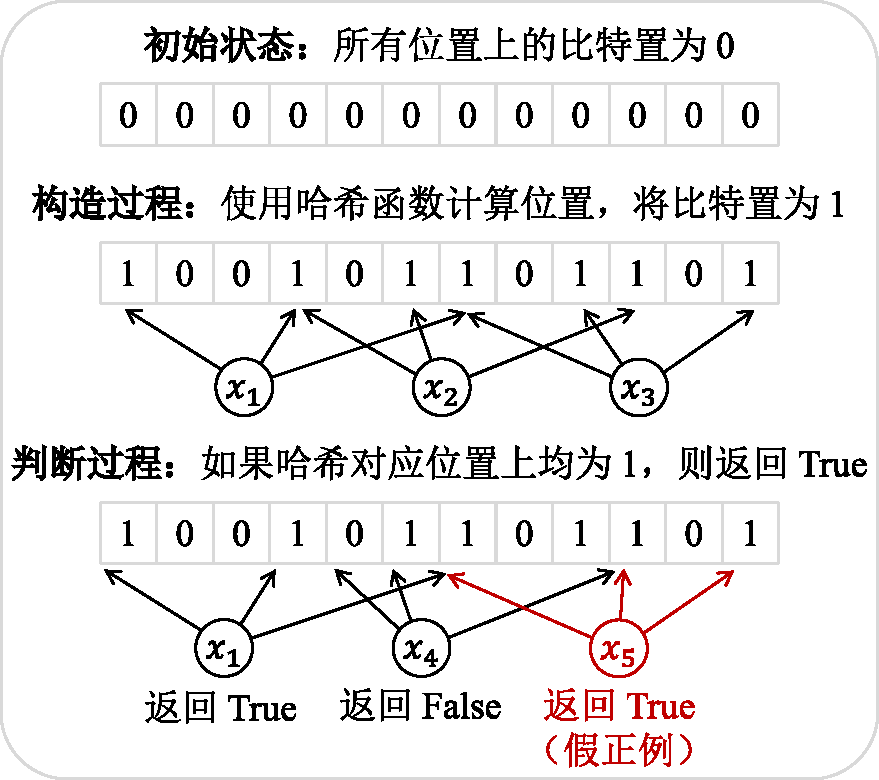
\includegraphics[width=0.7\textwidth]{figures/Bloom_filter.pdf}
  \caption{布隆过滤器示例($k=3$)}
  \label{fig:Bloom_example}
\end{figure}
以包含 $n$ 个元素的集合 $S=\{x_1, x_2, \dots, x_n\}$ 为例,假设构造的布隆过滤器长度为 $m$,使用的哈希函数为 $\{h_1, h_2, \dots, h_k\}$,其中每个哈希函数 $h_i:\{0,1\}^* \to [1, m]$ 为任意长度的输入到布隆过滤器上某一位置的映射。
首先我们将布隆过滤器 $m$ 个位置上的比特都置为 $0$,然后插入集合 $S$ 中的每一个元素。
在插入元素 $x$ 时,需要使用 $k$ 个哈希函数计算出 $k$ 个位置信息,即 $\{h_1(x),h_2(x),\dots, h_k(x)\}$。
最后将布隆过滤器上这 $k$ 个位置上的比特都置为 $1$。
% 一个包含 $n$ 个元素的集合,
在判断某个元素是否属于集合 $S$ 时,只需要计算该元素对应的 $k$ 个位置,然后检查这 $k$ 个位置上的比特是否都为 $1$。
只要有一个位置上出现了 $0$,那么判断结果就是不属于;否则,布隆过滤器认为该元素属于集合 $S$。
对于大小为 $n$ 的集合,其对应的的布隆过滤器需要 $O(nk)$ 的存储开销以及 $O(k)$ 的判断复杂度。

% 布隆过滤器是一种用于快速判断元素是否存在于某一集合的数据结构,它具有空间效率高、判断速度快的特点。
% 但是布隆过滤器也并不是
% 布隆过滤器的构造如图~\ref{fig:Bloom_example}~所示,它是使用 $k$ 个哈希函数 $\{h_1,\dots, h_k\}$ 构造的哈希表结构。
% 在初始状态,哈希表中所有所有位置上的比特都置为 $0$。
% 在构造过程中,对于每个在集合 $S$ 中的元素 $x$,只需要通过 $k$ 个哈希函数计算出对应的位置,并将这些位置上的比特置为 $1$。
% 首先使用这 $k$ 个哈希函数计算出 $k$ 个位置,然后对过滤器中该位置上的比特置为 $1$。
% 对于需要插入的元素,只需要通过 $k$ 个哈希函数计算出对应的位置,并将这些位置上的比特置为 $1$。
% 以大小为 $n$ 的集合 $S$ 为例,对应的布隆过滤器构造需要 $O(nk)$ 的存储开销以及 $O(k)$ 的判断复杂度。

% 布隆过滤器上分为插入(Insert)和查找(Lookup)两个算法,
% 在判断某个元素是否属于集合 $S$ 时,只需要通过哈希函数计算该元素的 $k$ 个位置,然后检查过滤器上这 $k$ 个位置上的比特是否全为 $1$。
% 如果是,返回 True,否则返回 False。
% 从布隆过滤器的构造可以看出,
% 假定有一个集合 $S$,其大小 $|S| = n$,
% 文献\cite{luo2019optimizing}:

% 布隆过滤器(Bloom filter,BF)是一种空间效率高的概率型数据结构,它可以用来快速判断元素是否属于某一集合。
% 布隆过滤器是由 0-1 比特组成的比特向量结构,包含插入(Insert)和查找(Lookup)两个基本算法。
% 以包含 $n$ 个元素的集合 $S=\{x_1, x_2, \dots, x_n\}$ 为例,假设构造的布隆过滤器长度为 $m$,使用的哈希函数为 $\{h_1, h_2, \dots, h_k\}$,其中每个哈希函数 $h_i:\{0,1\}^* \to [0, m-1]$ 为任意长度的输入到布隆过滤器上某一位置的映射。
% 首先我们将布隆过滤器 $m$ 个位置上的比特都置为 $0$,然后再插入集合 $S$ 中的每一个元素。
% 在插入元素 $x$ 时,需要使用 $k$ 个哈希函数计算出 $k$ 个位置信息,即 $\{h_1(x),h_2(x),\dots, h_k(x)\}$。
% 再将布隆过滤器上这 $k$ 个位置上的比特都置为 $1$。
% 一个包含 $n$ 个元素的集合,
% 在判断某个元素是否属于集合 $S$ 时,只需要计算该元素对应的 $k$ 个位置,然后检查这 $k$ 个位置上的比特是否都为 $1$。
% 只要有一个位置上出现了 $0$,那么判断结果就是不属于;否则,布隆过滤器认为该元素属于集合 $S$。

从布隆过滤器的构造和判断过程可以看出,如果一个元素属于集合 $S$,那么判断结果一定是正确的;但是如果一个元素不属于集合 $S$ (如图~\ref{fig:Bloom_example}~中的 $x_5$),布隆过滤器也有可能会认为该元素属于 $S$(输出结果为 True),此时判断错误的概率也称为假正例率(false positive rate)。
尽管布隆过滤器存在误判的问题,但在实际应用场景中,只要将误判率控制在较小的值,一般认为以一定的误判换取低空间开销和高效判断是值得的。

布隆过滤器的假正例率 $\epsilon$ 由布隆过滤器的长度 $m$,使用的哈希函数个数 $k$ 和集合中的元素个数 $n$ 所决定。
根据文献~\cite{luo2019optimizing}中的推导,理论上,误判率 $\epsilon$ 与它们的关系如公式~\eqref{eq:BF_FPR}所示:
\begin{equation}
    \epsilon = \left[ 1 - \left( 1 - \frac{1}{m} \right)^{nk} \right]^k \approx \left(1 - e^{-\frac{kn}m{}}\right)^k,
    \label{eq:BF_FPR}
\end{equation}
其中,$(1-1/m)^{nk}$ 近似成 $e^{-kn/m}$ 的形式。
为了尽可能降低误判率 $\epsilon$,那么就需要尽可能降低 $e^{-kn/m}$ 的值,这样一来,$k$ 的最优取值为:
\begin{equation}
    k_{opt}= \frac{m}{n}\ln 2 \approx \frac{9m}{13n}.
    \label{eq:BF_k}
\end{equation}
% 即 $m\approx 1.44 \cdot n \cdot k$
此时,误判率大约为 $\epsilon \approx 2^{-k}\approx 0.6185^{m/n}$。
通常在实际应用中的误判率要比理论分析上的更高,也有一些工作~\cite{bose2008falsepositive,christensen2010new}对误判率做了更精确的刻画。
% 从式~\ref{eq:BF_k}中可以推出,
布隆过滤器的优势主要体现在以下几个方面:
% 高效性主要体现在两个方面:
\begin{itemize}
    \item \textbf{较低的存储开销:}布隆过滤器的大小与元素的大小无关,只与集合中元素的数量有关。比如,当给定 $m$ 与 $n$ 的比值为 $5$ 时,根据公式~\eqref{eq:BF_k} 可以计算出需要的哈希函数数量为 $3$ 或 $4$。因为布隆过滤器中每个位置上存储的都是比特,所以整体长度也就是 $m$ 比特。
    \item \textbf{较高的判断效率:} 因为只需要检查 $k$ 个位置上的比特是否全为 $1$,因此检查一个元素的时间复杂度为 $O(k)$。相比于树形结构的查询复杂度$O(\log(n))$或列表结构的查询复杂度$O(n)$都要更低。
    % 而对于具体的布隆过滤器实例来说,$k$ 的值在初始化阶段就是常数,因此插入和查询的复杂度都为 $O(1)$。
    \item \textbf{不会漏判:} 尽管布隆过滤器在查询时会存在误判的情况,但是它不会出现漏判(假负例)的情况。也就是只要是布隆过滤器判断元素 $x$ 不属于 $S$,那么该论断一定是正确的。
\end{itemize}
% 布隆过滤器的挑战性问题:
但是,布隆过滤器也存在一些局限性:
\begin{itemize}
    \item \textbf{假正例率与过滤器长度:} 由于布隆过滤器中存在假正例的情况,而假正例率与过滤器的长度 $m$ 成反比。根据式~\ref{eq:BF_FPR},二者之间的关系为 $m\approx \frac{13}{9}nk \approx 1.44n\log_2(1/\epsilon)$。为了保证足够低的假正例率,就需要更大的 $m$ 来避免不同哈希映射导致的冲突。如此一来,过滤器的空间利用率就会降低。
    \item \textbf{动态性:} 布隆过滤器本身不支持元素的删除,因为如果是简单将需要删除元素所对应位置的比特置为 $0$,那么就会影响对其他元素的判断。
    \item \textbf{功能性:} 布隆过滤器只能判断元素是否属于某个集合,并不能检索元素对应的某一函数值或映射结果。
    % \item 实现,实际实现中需要考虑访问的优化,哈希计算的优化
    % \item 灵活性,哈希函数不能变,集合一开始就是确定的
    % \item 功能有限,只能做成员存在性测试
\end{itemize}

% 布隆过滤器本身是不支持删除的,因为如果是简单将需要删除元素所对应位置的比特置为 $0$,那么就会对其他元素的判断造成影响。
% 降低误判率的方法(思路):首先,

\section{定义及分类}\label{sec:defi_cate}

在介绍布隆过滤器相关衍生的数据结构之前,我们需要对这些数据结构进行分类。
为此,我们首先要对这些数据结构进行统一的定义。

\begin{definition}[过滤器]\label{def:filter}
    令 $\mathcal{U}$ 表示元素的集合,$\mathcal{H}$ 为哈希函数的集合。过滤器一般包含以下两个算法:
    % 的插入和查询算法如下所示。
    \begin{itemize}
    \item[$\circ$] $\mathsf{Construct}(S, \mathcal{H}) \to F/\perp$:输入集合 $S \subseteq \mathcal{U}$ 和预先给定的哈希函数集合 $\mathcal{H}$,输出构造的过滤器 $F$(或者以可忽略的概率输出错误指示符 $\perp$)。
    \item[$\circ$] $\mathsf{Evaluate}(x, \mathcal{H}, F) \to \mbox{True}/\mbox{False} $:输入元素 $x$,预先给定的哈希函数集合 $\mathcal{H}$,输出结果 True 或者 False。
    \end{itemize}

    \textbf{正确性:} 对于任意的 $S \subseteq \mathcal{U}$,都有:a).构建过程中,输出 $\perp$ 的概率是可忽略的;b).如果 $F \gets \mathsf{Construct}(S, \mathcal{H})$,且 $F \neq \perp$,那么在判断过程中,对于任意的 $x \in S$,$\Pr[\mathsf{Evaluate}(x, \mathcal{H}, F) = \mbox{True}] = 1$;对于任意 $x' \notin S$,$\Pr[\mathsf{Evaluate}(x, \mathcal{H}, F) = \mbox{True}]$ 为可忽略的。
\end{definition}
从以上定义中可以看出,如果一个元素在原本输入的集合中,那么过滤器在判断过程中一定能返回正确的结果,即过滤器中不存在假负例的情况;反之,如果一个元素不存在于输入的集合中,过滤器会大概率返回正确的结果,即过滤器中会存在一定的假正例率。

在判断过程中,需要使用 $\mathcal{H}$ 中的哈希函数计算出元素在 $F$ 中对应的位置,再对这些位置上记录的结果进行计算,最后根据计算结果与事先定义的 $f(x)$ 进行比较返回 $\mbox{Ture}$ 或者 $\mbox{False}$。
计算过程也被称为探测(probing),文献~\cite{dillinger2021ribbon}根据探测方式将过滤器分为以下三种类型:
\begin{itemize}
    \item \textbf{AND型:}在通过哈希函数计算出的位置中,如果所有位置上结果都与 $f(x)$ 相等,那么就输出 $\mbox{True}$;
    \item \textbf{OR型:}在通过哈希函数计算出的位置中,如果至少有一个位置上的值与 $f(x)$ 相等,那么就输出 $\mbox{True}$,否则输出 $\mbox{False}$。
    % 该类型的过滤器典型代表是布谷鸟过滤器~\cite{fan2014cuckoo},这种构造可以方便
    \item \textbf{XOR 型:}在通过哈希函数计算出的位置中,如果所有位置上值的异或结果与 $f(x)$ 相等,那么就输出 $\mbox{True}$,否则输出 $\mbox{False}$。
\end{itemize}
从以上分类可以看出,布隆过滤器的判断方式属于AND型。
% AND型的典型代表是布隆过滤器,
OR型的典型代表是布谷鸟过滤器(cuckoo filter)~\cite{fan2014cuckoo},这种构造的特点是支持元素的动态插入和删除。
XOR型的典型代表是异或过滤器(xor filter)~\cite{fan2014cuckoo},这类过滤器在结构上非常紧凑,具有较高的空间利用率,但受限于构建方式,这类构造通常不能支持元素的动态更新。

% 这里引用文献~\cite{2024YinSiJiHeYunSuanZhongDeGuanJianShuJuJieGouYanJiu}
不同的过滤器中对 $f(x)$ 的定义也略有不同。
一般来说分为以下几种情况:
\begin{itemize}
    \item $f(x)$ 为比特 $1$,最典型的是布隆过滤器,即要求 $x$ 对应所有位置上的结果都为 $1$,过滤器才会返回 $\mbox{True}$。
    % ,最典型的是布隆过滤器,即只有当通过哈希计算出的所有位置上都为 $1$,那么返回 $\mathsf{True}$。
    \item $f(x)$ 等于元素 $x$ 本身,典型的是混淆布隆过滤器 (garbled Bloom filter),即计算的结果为 $x$,过滤器才会返回 $\mbox{True}$。
    \item $f(x)$ 为 $x$ 的指纹(fingerprint),一般指的是 $x$ 的哈希值,典型代表为布谷鸟过滤器,即当有一个位置上的值与 $x$ 的指纹相同,过滤器才会返回 $\mbox{True}$。
    \item $f(x)$ 为任意函数,典型的是 Bloomier 过滤器,也就是说 $f(x)$ 的形式并不重要,或者说只要满足是 $x$ 一种映射关系即可。
\end{itemize}

从上述分类可以看出,对 $f(x)$ 的定义可以是简单的比特 $1$,也可以是关于 $x$ 的任意一种映射关系。
从另一个角度来看,键值型数据也可以看作是从键到值的映射,这样一来,键值型数据也可以编码成过滤器的形式。
按照这种想法得到的构造称作不经意键值存储(Oblivious Key-Value Store, OKVS),与过滤器不同,不经意键值存储返回的不是 $\mbox{True}$ 或者 $\mbox{False}$,而是与输入键相对应的值。
% 利用这种思路构造的结构称作不经意的键值存储(Oblivious Key-Value Store, OKVS),与过滤器不同,OKVS 返回的不是 $\mathsf{True}$ 或者 $\mathsf{False}$,而是与输入对应的数值。
不经意键值存储的定义如下:

\begin{definition}[不经意键值存储]\label{def:okvs}
    令 $\mathcal{K}$ 和 $\mathcal{V}$ 分别表示键和值的集合。不经意键值存储包含两个算法:
    \begin{itemize}
        \item[$\circ$] $\mathsf{Encode}(\{(x_1, y_1), (x_2, y_2), \dots, (x_n, y_n)\})$:输入一组键值对 $\{(x_i, y_i)\}_{i\in [n]}\subseteq \mathcal{K} \times \mathcal{V}$,输出编码结果 $D$ 或以可忽略的概率输出错误指示符 $\perp$。
        \item[$\circ$] $\mathsf{Decode}(D, k)$:输入编码结果 $D$ 和键 $k\in \mathcal{K}$,输出值 $v\in \mathcal{V}$。
    \end{itemize}

    \textbf{正确性:} 对于任意键值对集合 $A\subseteq \mathcal{K}\times \mathcal{V}$,如果 $\mathsf{Encode}(A) = D$ 且 $D\neq \perp$,那么对于任意的 $(k, v) \in A$,都有 $\mathsf{Decode}(D, k) = v$。

    \textbf{不经意性:} 随机给定两个不同的集合 $\mathcal{K}_0 = \{x_1^0, x_2^0, \dots, x_n^0\}$ 和 $\mathcal{K}_1 = \{x_1^1, x_2^1, \dots, x_n^1\}$,再随机构造集合 $\{y_i\}_{i\in [n]}\gets \mathcal{V}$,若 $D \neq \perp$,则分布 $\{D | y_i \gets \mathcal{V}, i\in [n], \mathsf{Encode}(\{(x_1^0, y_1), (x_2^0, y_2), \dots, (x_n^0, y_n)\})\}$ 与分布 $\{D | y_i \gets \mathcal{V}, i\in [n], \mathsf{Encode}(\{(x_1^1, y_1), (x_2^1, y_2), \dots, (x_n^1, y_n)\})\}$ 统计不可区分。

    对于部分安全需求较高的协议,不经意键值存储还需要满足随机性,即:

    \textbf{随机性:} 对于任意的集合 $A = \{(x_i, y_i)\}_{i\in [n]} \subseteq \mathcal{K} \times \mathcal{V}$ 和 $x' \notin \{x_1, x_2, \dots, x_n\}$,如果 $\mathsf{Encode}(A) = D$ 且 $D\neq \perp$,则 $\mathsf{Decode}(D, x')$ 的输出与随机选择的 $v\gets \mathcal{V}$ 统计不可区分。
\end{definition}

% 衡量指标:
我们主要考虑这些数据结构在存储和计算两个方面的性能。
% 评估以上数据结构的性能主要考虑存储和计算两个方面,
在存储开销方面,一是要衡量过滤器本身的长度,即 $m$ 的数值,我们一般使用负载因子(load factor) $\alpha = n/m$ 作为评估指标,即 $\alpha$ 越接近 $1$,说明空间利用率越高;二是需要衡量均摊空间开销(amortized space cost),即平均每个元素上在过滤器中所占用的存储空间。
在计算开销方面,我们主要分析构建/评估(或编码/解码)过程的复杂度。
% 基于以上讨论内容,
表~\ref{tab:construct}对本文中所介绍的过滤器以及不经意键值存储结构进行了总结。
% 接下来我们将对布隆过滤器衍生的数据结构进行详细介绍。
我们将在接下来的内容里对这些新型数据结构的构建方法进行详细介绍。

\begin{table}[ht]
  \centering
  \caption{不同过滤器及相关结构总结}
  \label{tab:construct}
  \begin{tabular}{cccc}
    \toprule
    名称  &  探测类型  &  $f(x)$  & 负载因子 $\alpha$ \\
    \midrule
    布隆过滤器  &  AND型  &  $1$ & $1.44\log_2(1/\epsilon)$  \\
    布谷鸟过滤器  &  OR型  &  $x$ 的指纹值 &   \\
    异或过滤器  &  XOR型  &  $x$ 的指纹值 &  \\
    二进制引信过滤器  & XOR型  &  $x$ 的指纹值 &  \\
    缎带过滤器 & XOR型 & $x$ 的指纹值 &  \\
    Bloomier 过滤器  &  XOR型  &  $f(x)$ & \\
    混淆布隆过滤器  &  XOR型  &  $x$ & \\
    随机带状不经意键值存储 &  XOR型  &  键 $x$ 对应的值 $y$ & \\
    \bottomrule
  \end{tabular}
\end{table}

\section{总结}

布隆过滤器是一种近似成员查询过滤器(approximate membership query filter),即以一定的误判率回答查询元素是否存在于集合中。
得益于其简洁的构造方式以及高效的判断性能,布隆过滤器的应用场景非常广泛。
除了前面提到的IP地址过滤、识别恶意邮件、DoS 和 DDos 攻击检测等场景之外,布隆过滤器及其衍生的数据结构也常被用于构造隐私保护相关协议~\cite{zhang2024survey}。
% 常用于对元素的存在性测试,在英文语境中,所谓``存在性测试''也被看作一种查询(m)
% 容易理解的构造以及
% 布隆过滤器的应用场景非常广泛,
% 由布隆过滤器衍生的数据结构大致有两个
布隆过滤器自提出后,各种变体形式层出不穷,如计数式布隆过滤器(counting Bloom filter)~\cite{lifan2000summary},压缩布隆过滤器(compressed Bloom filter)~\cite{mitzenmacher2002compressed},$d$-left 计数式布隆过滤器~\cite{bonomi2006improved},块布隆过滤器(blocked Bloom filter)~\cite{putze2009cache}等。
关于布隆过滤器的变体不在本文的讨论范围内,我们主要介绍布隆过滤器衍生出的新型数据结构,包括布谷鸟过滤器、异或过滤器、不经意键值存储等。
我们将在第~\ref{chp:data_structure}章对这些衍生数据结构进行详细介绍。
% 关于这些衍生数据结构我们将在第二章
最后,我们将在第~\ref{chp:application}章介绍这些数据结构在隐私保护方面的应用。
